\documentclass{standalone}


\usepackage{tikz}
\usepackage{pgfplots}
\usepackage{tkz-euclide}

\pgfplotsset{compat=1.6}

\usetikzlibrary{positioning,calc}
\usetikzlibrary{arrows} 
\usetikzlibrary{patterns} 
\usetikzlibrary{shapes}
\usetikzlibrary{decorations.pathmorphing}

\begin{document}

\def\BeforeLight{2}
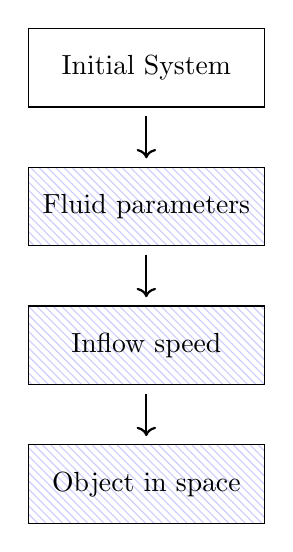
\begin{tikzpicture}
  % \draw[step=1cm, gray!20!white, very thin] (-5,-5) grid (5,5);

  
  \node[draw, minimum height=1cm,minimum width=3cm] at (0, 3) (n_1)             {Initial System};
  \node[draw, minimum height=1cm,minimum width=3cm, pattern=north west lines, pattern color=blue!20!white] (n_2) [below=0.75cm of n_1] {Fluid parameters};
  \node[draw, minimum height=1cm,minimum width=3cm, pattern=north west lines, pattern color=blue!20!white] (n_3) [below=0.75cm of n_2] {Inflow speed};
  \node[draw, minimum height=1cm,minimum width=3cm, pattern=north west lines, pattern color=blue!20!white] (n_4) [below=0.75cm of n_3] {Object in space};

  \draw [->, shorten >=3pt, shorten <=3pt, thick ] (n_1) edge (n_2);
  \draw [->, shorten >=3pt, shorten <=3pt, thick ] (n_2) edge (n_3);
  \draw [->, shorten >=3pt, shorten <=3pt, thick ] (n_3) edge (n_4);

  
  

\end{tikzpicture}


\end{document}

%%% Local Variables:
%%% mode: latex
%%% TeX-master: t
%%% End:
